\chapter{Untersuchung der Daten}

Um ein besseres Verst\"andnis f\"ur die Daten zu bekommen haben wir diese zun\"achst so zerlegt, dass die Blickdaten in kleineren Dateien gespeichert wurden, die nur noch jeweils die Daten f\"ur einen Versuch enthalten. Die Targetdateien wurden ebenfalls so zerlegt, dass kleine Dateien entstanden, die die Daten f\"ur einen Versuch pro Versuchsperson enthalten.
Die Daten wurden dann entsprechend neustrukturiert gespeichert, sodass es zu jeder Versuchsperson einen Ordner gibt, in dem die Versuche enthalten sind, in denen wiederum die Durchg\"ange enthalten sind. Dabei entstand die in Abbildung \ref{fig:Ordnerstruktur} dargestellte Struktur.

\begin{figure}[H]
	\noindent \begin{centering}
		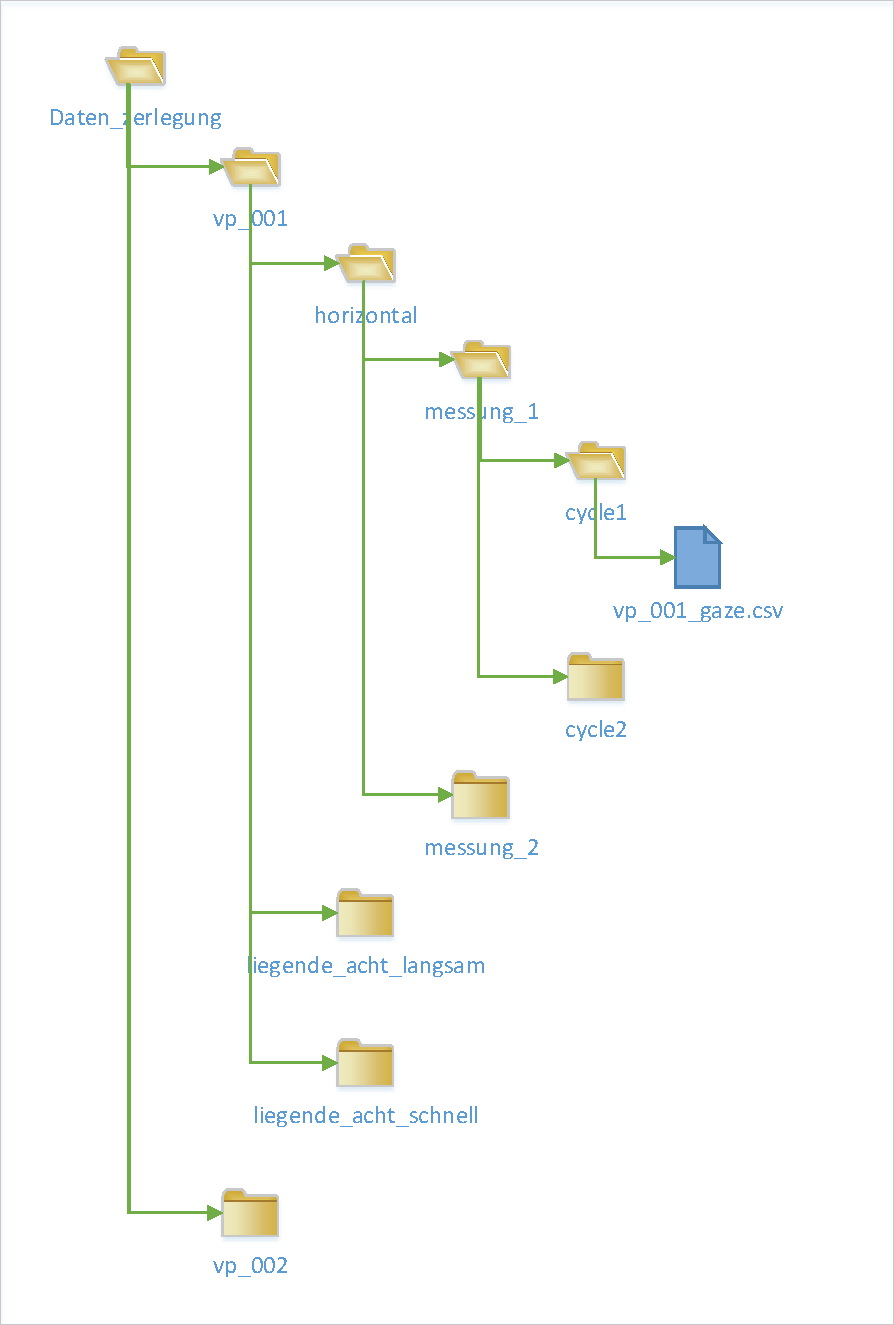
\includegraphics[width=15cm]{pics/Darstellung-Ordnerstruktur.pdf}
		\par\end{centering}
	\caption{\label{fig:Ordnerstruktur}Darstellung Ordnerstruktur}
\end{figure}

Die Versuche wurden dann visualisiert. \\
Durch die Visualisierung konnte man erkennen, dass die Targetdateien und die Blickdateien auf unterschiedlichen Koordinatensystemen beruhen. \\
Abbildung \ref{fig:Visualisierung} zeigt ein Beispiel f\"ur die Visualisierung der liegenden acht langsam.

\begin{figure}[H]
	\noindent \begin{centering}
		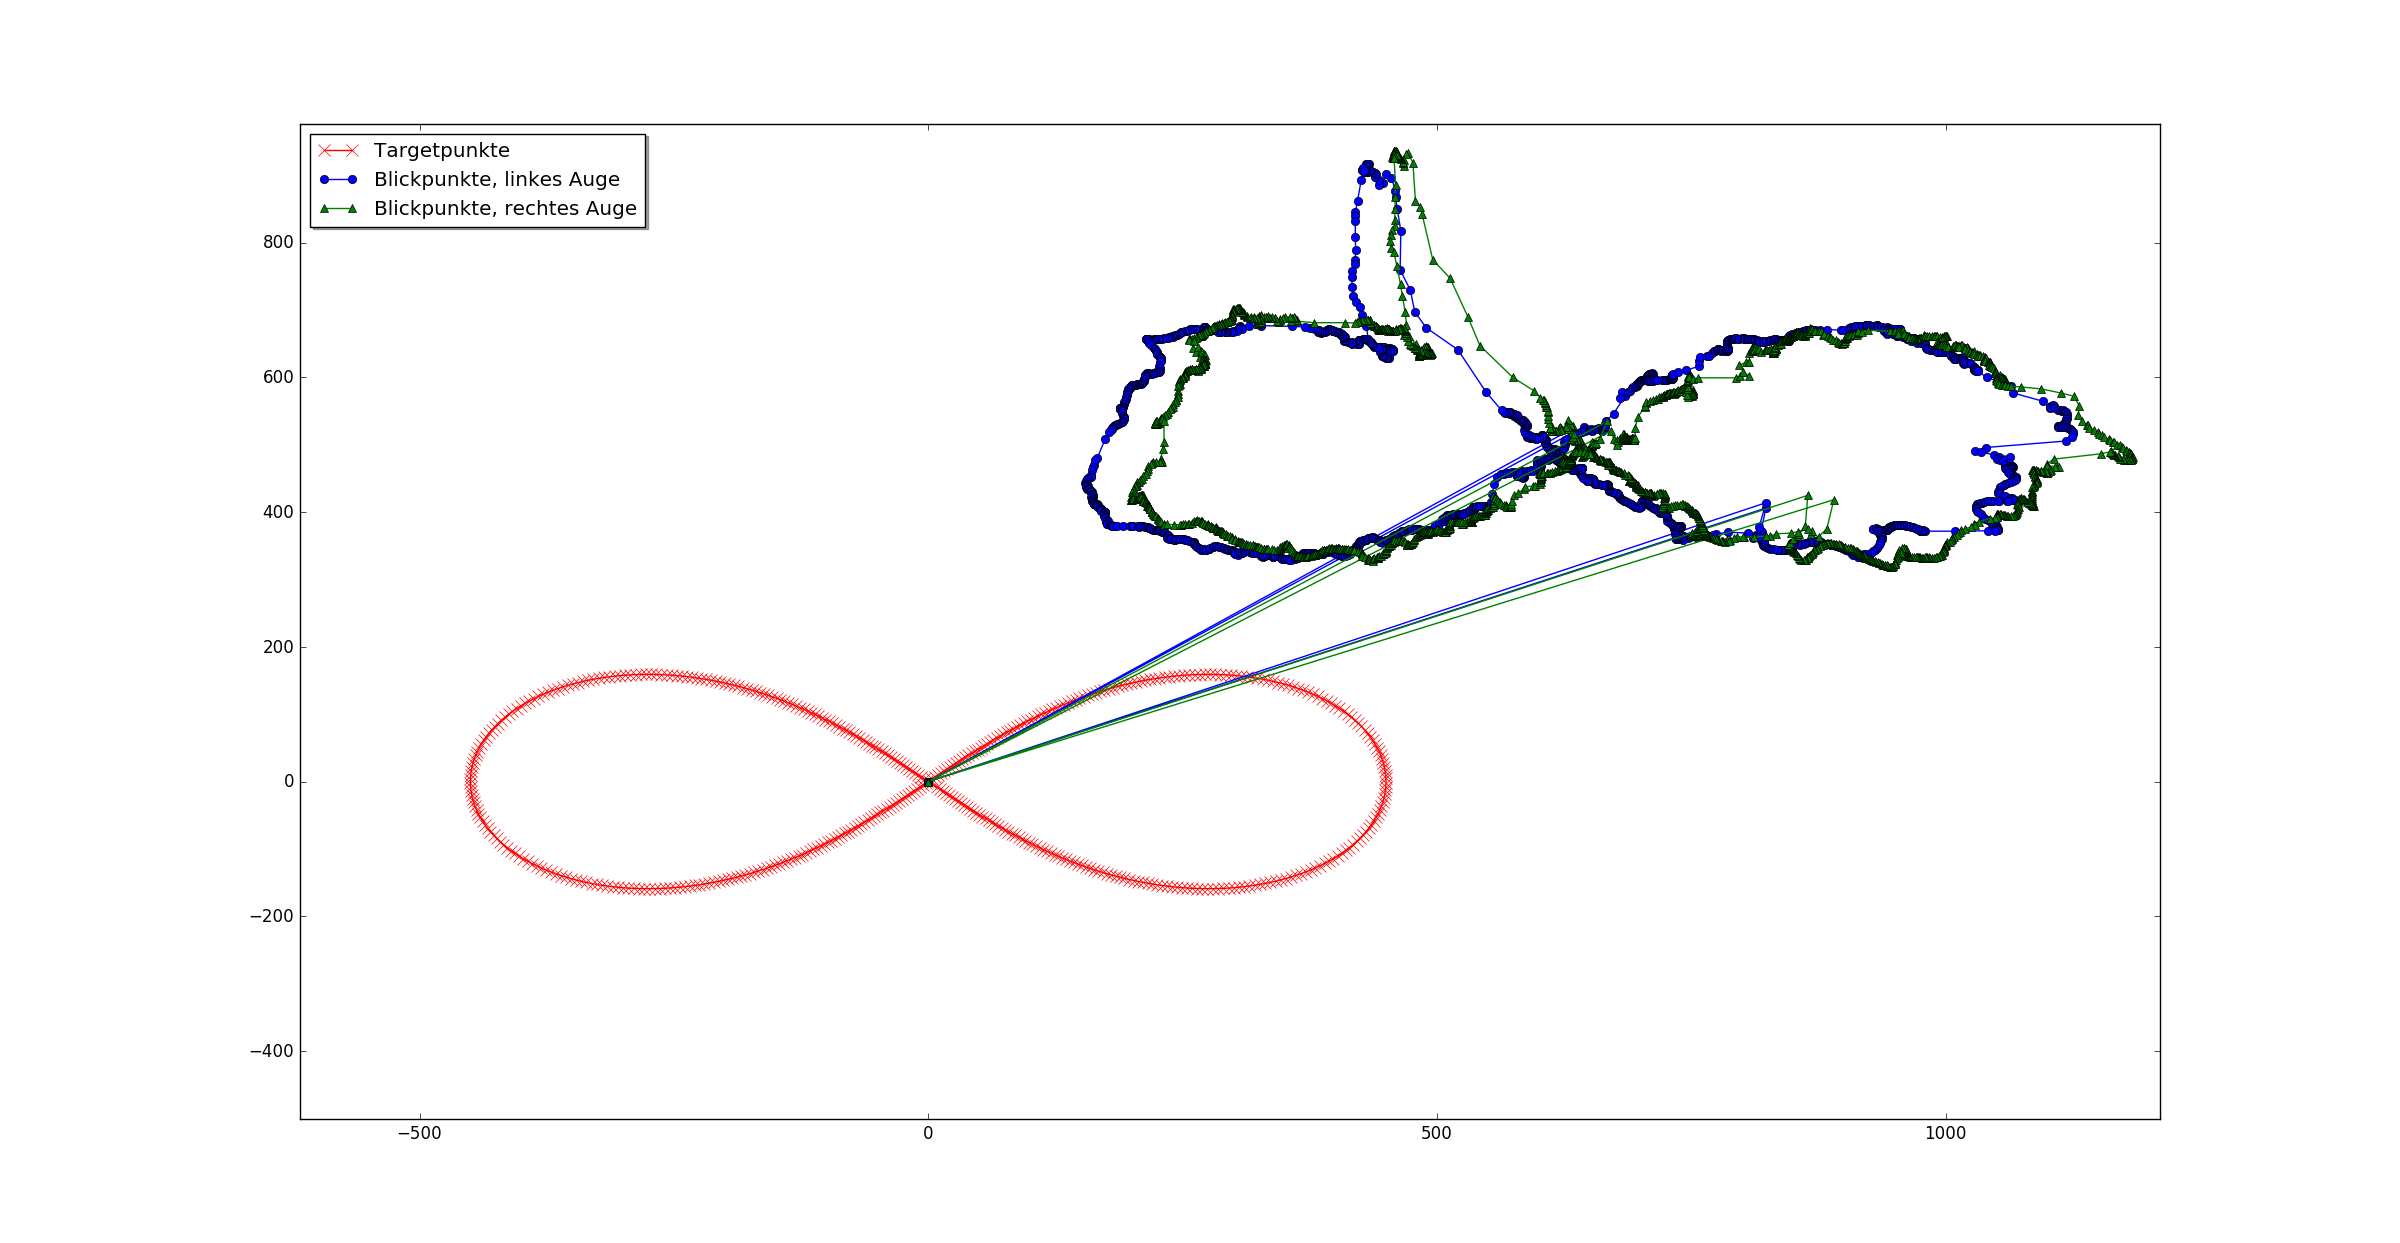
\includegraphics[width=15cm]{pics/figure_1-1.png}
		\par\end{centering}
	\caption{\label{fig:Visualisierung}Visualisierung der Blickpunkte}
\end{figure}